\newcommand{\nom}{Porte conteneur}
\newcommand{\sequence}{03}
\newcommand{\num}{04}
\newcommand{\type}{TD}
\newcommand{\descrip}{Résolution d'un problème en utilisant des méthodes algorithmiques}
\newcommand{\competences}{Alt-C3: Concevoir un algorithme répondant à un problème précisément posé}

\documentclass[10pt,a4paper]{article}
  \usepackage[french]{babel}
  \usepackage[utf8]{inputenc}
  \usepackage[T1]{fontenc}
  \usepackage{xcolor}
  \usepackage[]{graphicx}
  \usepackage{makeidx}
  \usepackage{textcomp}
  \usepackage{amsmath}
  \usepackage{amssymb}
  \usepackage{stmaryrd}
  \usepackage{fancyhdr}
  \usepackage{lettrine}
  \usepackage{calc}
  \usepackage{boxedminipage}
  \usepackage[french,onelanguage, boxruled,linesnumbered]{algorithm2e}
  \usepackage[colorlinks=false,pdftex]{hyperref}
  \usepackage{minted}
  \usepackage{url}
  %\usepackage[locale=FR]{siunitx}
  \usepackage{multicol}
  \makeindex

  %\graphicspath{{../Images/}}

  \renewcommand\listingscaption{Programme}

  %\renewcommand{\thechapter}{\Alph{chapter}}
  \renewcommand{\thesection}{\Roman{section}}
  %\newcommand{\inter}{\vspace{0.5cm}%
  %\noindent }
  %\newcommand{\unite}{\ \textrm}
  \newcommand{\ud}{\mathrm{d}}
  \newcommand{\vect}{\overrightarrow}
  %\newcommand{\ch}{\mathrm{ch}} % cosinus hyperbolique
  %\newcommand{\sh}{\mathrm{sh}} % sinus hyperbolique

  \textwidth 160mm
  \textheight 250mm
  \hoffset=-1.70cm
  \voffset=-1.5cm
  \parindent=0cm

  \pagestyle{fancy}
  \fancyhead[L]{\bfseries {\large PTSI -- Dorian}}
  \fancyhead[C]{\bfseries{{\type} \no \num}}
  \fancyhead[R]{\bfseries{\large Informatique}}
  \fancyfoot[C]{\thepage}
  \fancyfoot[L]{\footnotesize R. Costadoat, J. Genzmer, W. Robert}
  \fancyfoot[R]{\small \today}
  
  \definecolor{bg}{rgb}{0.5,0.5,0.5}
  \definecolor{danger}{RGB}{217,83,79}
  
  \fancypagestyle{correction}{%
  \fancyhf{}
  \lhead{\colorbox{danger}{\begin{minipage}{0.65\paperwidth} \textcolor{white}{\textbf{Correction}} \end{minipage}} }
  \rhead{
\includegraphics[width=2cm]{../../img/logo}}
  \lfoot{Juliette Genzmer, Willie Robert, Renaud Costadoat}
  \rfoot{\colorbox{danger}{\begin{minipage}{0.6\paperwidth} \begin{flushright}\textcolor{white}{\textbf{Correction}}\end{flushright} \end{minipage}} }}

  
  % macro Juliette
  
\usepackage{comment}   
\usepackage{amsthm}  
\theoremstyle{definition}
\newtheorem{exercice}{Exercice}
\newtheorem*{rappel}{Rappel}
\newtheorem*{remark}{Remarque}
\newtheorem*{defn}{Définition}
\newtheorem*{ppe}{Propriété}
\newtheorem{solution}{Solution}


\begin{document}

\excludecomment{solution}

\begin{document}

\section{Présentation}

Un paysan possède un âne pour lequel il réserve un pré de longueur $L=20m$ et de largeur $l=20m$. L'âne est attaché à un poteau par une corde de longueur $c=2m$. De temps en temps, le propriétaire de l'âne est obligé de venir déplacer le poteau car l'âne a mangé toute l'herbe qu'il pouvait atteindre.

Il se rend compte que le choix de l'emplacement du poteau est important car parfois, après avoir effectué plusieurs déplacements, les zones où il reste de l'herbe sont éparpillées et de faible taille ce qu'il fait qu'il doit venir déplacer souvent l'âne.

Enfin, il est absolument interdit que l'âne ait la possibilité de manger l'herbe du pré voisin car le paysan n'en est pas le propriétaire.

Résumé des contraintes:
\begin{itemize}
 \item L'âne ne doit pas aller en dehors de ce pré,
 \item Le propriétaire doit effectuer le minimum de déplacements de poteau,
 \item La surface d'herbe non mangée par l'âne ne doit pas excéder 15\% de la surface du terrain.
\end{itemize}

\textbf{Objectif:} L'objectif de cette étude va être de proposer les positions des poteaux au paysan afin de respecter ces contraintes.

Le DM devra être rendu au format numérique, par mail ou sur une clef USB.

Dans un premier temps, nous allons suivre une grille afin de placer les poteaux.

\section{Fonction $Manger$}

Soient $(x,y)$, les coordonnées du poteau dans le repère $O(\overrightarrow{x}, \overrightarrow{y})$, lié au champ.

Soit $(i,j)$ les coordonnées d'un point M du champ dans le repère $O(\overrightarrow{x}, \overrightarrow{y})$.

\paragraph{Question 1:} Donner l'inéquation vérifiée par $i$, $j$, $x$, $y$ et $c$ correspondant aux points $M(i,j)$ accessibles par l'âne lorsque le poteau est en $(x,y)$ pour une corde de longueur $c$.

~\

Pour simuler numériquement le problème, le champ va être découpé en petits carrés de $10cm$ de côté. Chaque carré a pour centre le point $M(i,j)$ et on considère que le carré est entièrement mangé si son centre $M(i,j)$ est accessible à l'âne.

La matrice \verb? pre ? va servir de $map$ pour déterminer si une zone a été broutée ou pas. En effet, la composante \verb? pre[i,j] ? sera égale à :
\begin{itemize}
 \item $0$, si la zone n'a pas été parcourue par l'âne,
 \item $1$, si la zone a été parcourue par l'âne une fois,
 \item $2$, si la zone a été parcourue par l'âne plus d'une fois.
\end{itemize}

\begin{center}
 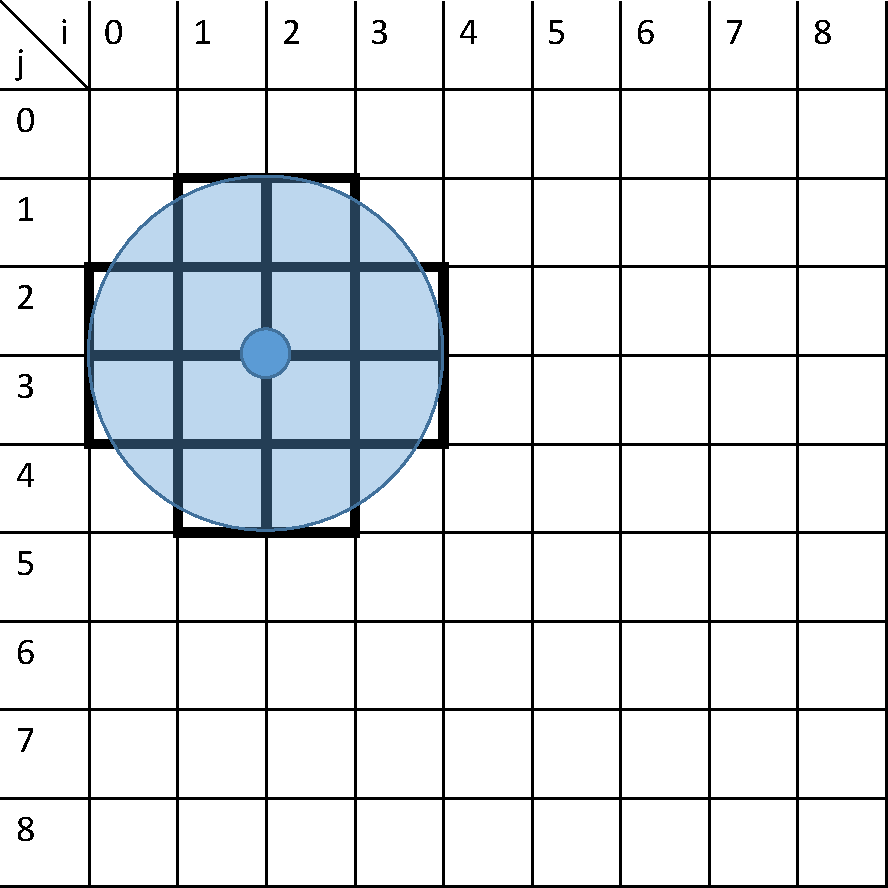
\includegraphics[width=0.5\linewidth]{img/Figure1}
\end{center}

\paragraph{Question 2:} Définir une fonction \verb? manger(x,y)? qui parcourt chacun des carrés de coordonnées $(i,j)$, teste si il est accessible à l'âne et si il a déjà été mangé, et qui modifie la matrice \verb? pre ?. Les entrées de cette fonction sont les coordonnées $(x,y)$ du poteau. 

\paragraph{Question 3:} Proposer un algorithme qui fait parcourir au poteau le pré en commençant par la position $x_0=20dm$ et $y_0=20dm$ en se décalant à chaque fois d'un intervalle $e$ et remplissant la matrice \verb? pre?. On prendra pour commencer $e$ égal à $35dm$ (on le fera varier par la suite).

\section{Fonction $Analyse$}

La fonction analyse va traiter la matrice \verb? pre ? générée précédemment. Si vous n'avez pas réussi à déterminer la matrice \verb? pre ?, le fichier \verb? Pre.txt ?, vous permet d'en générer une. Il est écrit sous la forme \verb? i,j,pre[i,j] \n ?. Il est disponible sur le forum.

\paragraph{Question 4:} Créer une fonction \verb? analyse ? qui en parcourant la liste \verb? pre ?, créer une liste:
\begin{itemize}
 \item \verb? x1 ? qui renvoie l'ensemble des i parcourus dans le sens des $i$ croissants puis des $j$ croissants lorsque \verb? pre[i,j]=1 ?,
 \item \verb? y1 ? qui renvoie l'ensemble des j parcourus dans le sens des $i$ croissants puis des $j$ croissants lorsque \verb? pre[i,j]=1 ?,
 \item \verb? x2 ? qui renvoie l'ensemble des i parcourus dans le sens des $i$ croissants puis des $j$ croissants lorsque \verb? pre[i,j]=2 ?,
 \item \verb? y2 ? qui renvoie l'ensemble des j parcourus dans le sens des $i$ croissants puis des $j$ croissants lorsque \verb? pre[i,j]=2 ?.
\end{itemize}

Cette fonction devra aussi retourner le nombre de $1$ dans la matrice \verb? pre ? et le nombre de $2$ dans la matrice \verb? pre ?.

\section{Fonction $Pourcent$}

\paragraph{Question 5:} Créer une fonction \verb? pourcent ? qui pour une entrée $k$ (représentant le nombre de $1$ plus le nombre de $2$ dans la matrice \verb? pre ?) retourne le pourcentage que ce nombre $k$ représentante par rapport à l'ensemble des éléments de la matrice \verb? pre ?

\paragraph{Question 6:} Quel résultat vous donne la fonction \verb? pourcent ?, ce résultat respecte-t-il le cahier des charges ?

\section{Tracé de la réponse et optimisation}

Le code suivant va vous permettre de tracer le résultat obtenu.

\begin{minipage}{0.45\linewidth}
\begin{verbatim}]
import matplotlib.pyplot as plt

plt.scatter(x1,y1,s=1,color='green')
plt.scatter(x2,y2,s=1,color='red')
plt.axis('equal')
plt.xlim(0, long)
plt.ylim(0, larg)
plt.show()
\end{verbatim}
\end{minipage}\hfill
\begin{minipage}{0.45\linewidth}
\begin{center}
 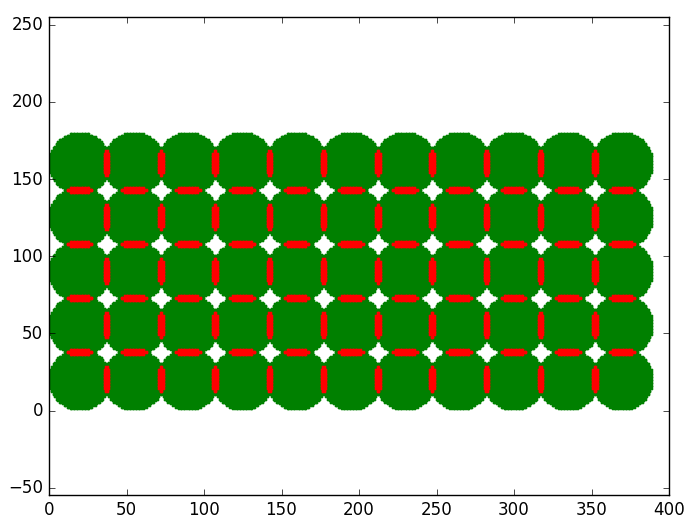
\includegraphics[width=0.8\linewidth]{img/Figure2}
\end{center}
\end{minipage}

Sur cette figure, on trouve en vert l'herbe broutée une seule fois, en rouge, celle broutée deux fois et en blanc celle qui n'a pas été broutée.

\paragraph{Question 7:} Modifier la valeur de $e$ afin de respecter le cahier des charges.

\paragraph{Question 8:} Donner le pourcentage de zones \og rouges \fg  par rapport à la surface du pré avec cette nouvelle valeur de $e$.

\section{Nouvelle solution (facultatif)}

Dans cette solution proposer une disposition en quinconce de la position du poteau et tenter d'améliorer les performances précédentes.

\begin{center}
 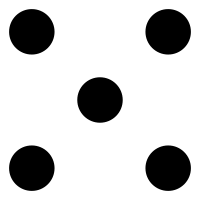
\includegraphics[width=0.2\linewidth]{img/quinconce}
\end{center}

\paragraph{Question 9:} Donner les nouvelles valeurs trouvées pour les questions 6 et 8. Que concluez-vous quant à cette simulation.

\begin{solution}

\newpage

\section{Correction}

\paragraph{Question 1:} $(i-x)^2+(j-x)^2\leq c^2$

\paragraph{Question 2:} 
\begin{verbatim}
def manger(x,y):
    for i in range(long):
        for j in range(larg):
            if (i-x)**2+(j-y)**2<corde**2 and pre[i,j]!=0:
                pre[i,j]=2
            if (i-x)**2+(j-y)**2<corde**2 and pre[i,j]==0:
                pre[i,j]=1
    return pre
\end{verbatim}

\paragraph{Question 3:} 

\begin{verbatim}
def calcul_classique(x0,y0,inc):
    x=x0
    y=y0
    while y+corde < larg:
        while x+corde < long:
            pre=manger(x,y)
            x=x+inc
        x=x0
        y=y+inc
    return pre
\end{verbatim}

\paragraph{Question 4:} 

\begin{verbatim}
def analyse(pre):
    k,h=0,0    
    x1,y1,x2,y2 = [],[],[],[]
    for i in range(long):
        for j in range(larg):
            if pre[i,j] == 1:
                k=k+1
                x1.append(i)
                y1.append(j)
            if pre[i,j] == 2:
                h=h+1
                x2.append(i)
                y2.append(j)
    return x1,y1,x2,y2,k,h
\end{verbatim}

\paragraph{Question 5:} 

\begin{verbatim}
def pourcent(k):
    return 100*(k)/(long*larg)
\end{verbatim}

\paragraph{Question 6:} La réponse est 78\%, cela ne respecte pas le cahier des charges.

\paragraph{Question 7:} La valeur de $e=29$ convient.

\paragraph{Question 8:} Pour $e=29$, on obtient:
\begin{itemize}
 \item Surface couverte 86\%,
 \item Surface couverte 2 fois 34\%.
\end{itemize}

Cela respecte le cahier des charges.

\paragraph{Question 9:}

\begin{verbatim}
def calcul_quinconce(x0,y0,inc):
    u=0
    x=x0
    y=y0
    while y+corde+inc/2 < larg:
        while x+corde < long:
            u=u+1
            if (u % 2 == 0):
                pre=manger(x,y+inc/2)
            else:
                pre=manger(x,y)
            x=x+inc
        x=x0
        u=0
        y=y+inc
    return pre
\end{verbatim}

Ici le résultat obtenu pour $e=34.9$ est :
\begin{itemize}
 \item Surface couverte 81\%,
 \item Surface couverte 2 fois 4\%.
\end{itemize}

Même si la zone \og rouge \fg a diminué, le cahier des charges pourra difficilement être respecté avec cette simulation.
\end{solution}

\end{document}
